
\section{ソフトの構成}
\subsection{外部データの読み込み部}
\subsubsection{read\_pos}\begin{lstlisting}[style=customRuby,basicstyle={\scriptsize\ttfamily}]
def read_pos(lines, init_line=8)
  lattice, atom, poscar = [],[],[]
  lines[2..4].each{|line| lattice << line.scanf("%f %f %f\n")  }
  lines[init_line..lines.length+1].each{|line| atom << line.scanf("%f %f %f\n") }

  atom.each{|i_atom|
    pos=[0.0,0.0,0.0,0.0]
    i_atom.each_with_index{|atom_j,j|
      lx,ly,lz=lattice[j]
      pos[0] += atom_j*lx
      pos[1] += atom_j*ly
      pos[2] += atom_j*lz
    }
    poscar << pos
  }
  return poscar
end
\end{lstlisting}
関数read\_posは,外部データをARGVで読み込んでいるファイルlinesを受け取って.配列に格納する機能を果たしている.
コードの3行目では,linesの2行目から4行目の値を読み込んで配列lattticeに格納しており,その後にlinesの8行目から最後の行までの読み込んだ値を配列atomsに格納している.
6行目からは,配列atomsをeach文で繰り返し,その中で配列lattice内に格納された各々の座標をlx,ly,lzと定義している.
定義した格子の各座標と原子の各座標の積をとって原子配列の座標をもとめ,その値を配列poscarに格納している.
原子座標ファイルPOSCAR\_2223において,配列poscarに格納された原子座標は以下の実行結果により表示される.
\begin{lstlisting}[style=,basicstyle={\scriptsize\ttfamily}]
[Narita-no-MacBook-Air:~/boundary/narita/view] nari% ruby final.rb POSCAR_2223 POSCAR_2223_4
[5.75101295815, 0.0, 0.0, 0.0]
[7.668017277916733, 0.6390014395849836, 2.020699977875, 0.0]
[3.834008638383265, 0.6390014395849836, 2.020699977875, 0.0]
[7.029015837611088, 2.556005758968566, 0.0, 0.0]
[4.473010078688911, 2.556005758968566, 0.0, 0.0]
[5.75101295815, 0.0, 4.04139995575, 0.0]
[7.668017277916733, 0.6390014395849836, 6.062099933625, 0.0]
[3.834008638383265, 0.6390014395849836, 6.062099933625, 0.0]
[7.029015837611088, 2.556005758968566, 4.04139995575, 0.0]
[4.473010078688911, 2.556005758968566, 4.04139995575, 0.0]
[6.390014398455645, 4.473010078352149, 2.020699977875, 0.0]
[5.112011517844354, 4.473010078352149, 2.020699977875, 0.0]
[6.390014398455645, 4.473010078352149, 6.062099933625, 0.0]
[5.112011517844354, 4.473010078352149, 6.062099933625, 0.0]
...
[1.2780028794610885, 5.751012958150748, 6.062099933625, 0.0]
\end{lstlisting}
\subsection{原子座標の計算部}
\subsubsection{identical\_atoms}\begin{lstlisting}[style=customRuby,basicstyle={\scriptsize\ttfamily}]
def identical_atom(i_atom,j_atom)
  dist=0.0
  3.times{|i| dist += (i_atom[i]-j_atom[i])**2  }
  return true if Math.sqrt(dist)<0.5
  return false
end
\end{lstlisting}
関数identical\_atomsは,2つのPOSCARファイルに含まれる各々の原子座標の距離を求めて,ある値の大小比較をおこなって真偽を判定する機能を果たしている.
具体的に,ファイル内のある原子i\_atomともう片方のファイル内にある原子j\_atomの距離が0.5より小さい値であればtrueと判定して返す.
そうでなければ,falseを返して終了する.

\subsubsection{mk\_deleted\_atom}\begin{lstlisting}[style=customRuby,basicstyle={\scriptsize\ttfamily}]
def mk_deleted_atom
  mark=[]
  j_max = $pos_after.length
  $pos_before.each_with_index{|i_atom,i|
    update_num=0
    $pos_after.each_with_index{|j_atom,j|
      break if identical_atom(i_atom,j_atom)
      update_num = j
    }
    mark << $pos_before[i] if update_num==(j_max-1)
  }
  return mark
end
\end{lstlisting}
関数mk\_deleted\_atomは,原子削除をおこなう前後のPOSCARファイルを比較して削除された原子のみを別の配列に格納する機能を果たしている.
関数内では,始めに更新するための値update\_numを0と定め,2つのPOSCARファイルをeach文で繰り返しながら,identical\_atomでtrueとして返されたものを配列markの方へ格納している.
POSCAR\_2223において,配列markに格納された原子座標が以下の実行結果である.
\begin{lstlisting}[style=,basicstyle={\scriptsize\ttfamily}]
[Narita-no-MacBook-Air:~/boundary/narita/view] nari% ruby final.rb POSCAR_2223 POSCAR_2223_4
[[6.390014398455645, 4.473010078352149, 2.020699977875, 0.0] 
[5.112011517844354, 4.473010078352149, 6.062099933625, 0.0] 
[10.863024475994353, 3.8340086387671652, 0.0, 0.0]
 [0.6390014403056455, 3.8340086387671652, 0.0, 0.0] 
[10.863024475994353, 3.8340086387671652, 4.04139995575, 0.0]]
\end{lstlisting}
\subsection{粒界原子の描画部}
\subsubsection{draw\_backcolor, draw\_axes}\begin{lstlisting}[style=customRuby,basicstyle={\scriptsize\ttfamily}]
def draw_backcolor
  $context.set_source_rgb(0.8, 0.8, 0.8)
  $context.rectangle(0, 0, $width, $height)
  $context.fill
end

def draw_axes
  $context.set_source_rgb(0, 0, 0)
  [[0,1],[1,0]].each{|line|
    x,y=line[0],line[1]
    [[0,0],[$cx,0],[0,$cy]].each{|c_x,c_y|
      $context.move_to($mv+c_x,$mv+c_y)
      $context.line_to($mv+c_x+x*$scale,$mv+c_y+y*$scale)
      $context.stroke
    }
  }
end
\end{lstlisting}
関数draw\_backcolorは,原子配列の背景を描画しており,SVGで表示する画面のサイズを明確にするために作成している.
また,関数draw\_axesは,原子配列における縦軸と横軸を描画しており,each文で3つ平面に必要な軸をまとめて出力できるようにしている.

\subsubsection{open\_circle}\begin{lstlisting}[style=customRuby,basicstyle={\scriptsize\ttfamily}]
def open_circle
  z_layer=[]
  layer_max, layer_min = $pos_max[2], 0.0
  bound=(layer_max - layer_min )/($denominator-1)
  num,j = layer_min, 0
  $diff = 0.15
  while num <= layer_max do
    z_layer[j] = num
    num += bound
    j += 1
  end
  return z_layer
end
\end{lstlisting}
関数open\_circleは,白抜きする層の座標を計算して配列に格納している.
3行目のlayer\_maxは,関数find\_maxで得た原子のz座標の最大値をとっており,layer\_minはz座標の最小値として初期値0を与えている.
その後に挿入されているboundは,各層の倍数の値をとっている.
この倍数値は,z座標の最大値と最小値の差をとって,その値を関数main\_drawで読み込んだ分母の値denominatorで割ることにより結果を得ている.
while文では,layer\_minからlayer\_maxまでの範囲で倍数値boundを加算させていき,加えていった各数値を配列z\_layerに格納している.
また,コード内のdiffは,白抜きする原子座標の範囲の近似値を示している.

\subsubsection{pos\_y}\begin{lstlisting}[style=customRuby,basicstyle={\scriptsize\ttfamily}]
def pos_y(pos, c_y, index, select)
  dy = select == 0 ? pos[index] : $pos_max[index]-pos[index]
  return $mv+c_y+$adjust*dy
end
\end{lstlisting}
関数pos\_yは,x−y平面でのy軸を逆転させる計算をおこなっている.
具体的に,関数draw\_each\_planeの中のselで描画する平面の判定した結果をもらい,x−y平面ならば,関数find\_maxにより得たy座標の最大値から各y座標を差分し,その値をdyへ与えている.
x−y平面以外であれば,そのままの値を返している.

\subsubsection{draw\_each\_plane}\begin{lstlisting}[style=customRuby,basicstyle={\scriptsize\ttfamily}]

def draw_each_plane(ind_1,ind_2,c_x,c_y)
  rr = 2
  sel = (ind_1==0 and ind_2==1)? 1 : 0
  [[$deleted_atoms,[1,0,0],rr*1.3],[$pos_after,[0,0,1],rr]].each{|atoms_color|
    $context.set_source_rgb(atoms_color[1])
    radius = atoms_color[2]
    atoms_color[0].each{|pos|
      if $numerator == 0 then
        $context.circle($mv+c_x+$adjust*pos[ind_1],pos_y(pos,c_y,ind_2,sel), radius)
        $context.fill
      else
        if pos[2] < open_circle[$numerator-1]+$diff and open_circle[$numerator-1] - $diff < pos[2] then
          $context.circle($mv+c_x+$adjust*pos[ind_1],pos_y(pos,c_y,ind_2,sel), radius*1.7)
          $context.stroke
          $context.set_line_width(0.5)
        else
          $context.circle($mv+c_x+$adjust*pos[ind_1],pos_y(pos,c_y,ind_2,sel), radius)
          $context.fill
        end
      end
    }
  }

  if $pos_before.size==$pos_after.size
    $context.set_source_rgb(0, 0.8, 0)
    (0..$pos_before.length-1).each{|i|
      $context.move_to($mv+c_x+$adjust*$pos_before[i][ind_1],pos_y($pos_before[i],c_y,ind_2,sel))
      $context.line_to($mv+c_x+$adjust*$pos_after[i][ind_1],pos_y($pos_after[i],c_y,ind_2,sel))
      $context.stroke
    }
  end
end
\end{lstlisting}
関数draw\_each\_planeでは,描画する原子の位置,色,大きさを定め,さらに原子の白抜き判定もおこなっている.
2行目のrrの値は,原子の半径値を示している.3行目では,atoms\_colorの配列を組み,削除の有無によって原子の色と大きさを変えるようにしている.
if-else文で,分子の値numeratorが0であるかを判定しており,真であれば白抜きなしの原子配列を描画する.
分子の値numeratorが0でない,すなわち指定した層の値がnumeratorに入力されているのならば,関数open\_circleで各層の値を格納しているz\_layerの配列番号を指定し,近似値diffで範囲を求めて指定した層の白抜き描画をおこなっている.
また,24行目のif文では,読み込んだ2つの原子配列ファイルPOSCARのデータサイズを比較しており,同じサイズであるならば,2つのファイルにおける各原子間の距離を線で表示するようにしている.

\subsubsection{draw\_atoms}\begin{lstlisting}[style=customRuby,basicstyle={\scriptsize\ttfamily}]
def draw_atoms
  draw_each_plane(0,1,0,0)    
  draw_each_plane(0,2,0,$cy)   
  draw_each_plane(1,2,$cx,$cy) 
end
\end{lstlisting}
関数draw\_atomsでは,前の関数draw\_each\_planeで設定した原子配列を三面図の規定位置にそれぞれ描画するようにしている.
具体的に,x−y平面を平面図として第二象限,x−z平面を正面図として第三象限,y−z平面を側面図として第四象限に出力させている.

\subsubsection{find\_max}\begin{lstlisting}[style=customRuby,basicstyle={\scriptsize\ttfamily}]
def find_max(pos)
  max = [0,0,0]
  [0,1,2].each{|ind|
    pos.length.times {|i| max[ind] = pos[i][ind] if max[ind] < pos[i][ind] }
  }
  return max
end
\end{lstlisting}
関数find\_maxは,原子の各座標の最大値を探索する機能を果たしている.
配列posには,関数read\_posで(x,y,z)=(0,1,2)としてそれぞれの値を読み込んでおり,隣接する値の大小比較をおこなって,各座標の最大値を配列maxに格納している.

\subsubsection{main\_draw}\begin{lstlisting}[style=customRuby,basicstyle={\scriptsize\ttfamily}]
def main_draw(file1,file2, layer, model_scale = 10)
  lines1 = File.readlines(file1)
  lines2 = File.readlines(file2)
  if layer != nil then
    tmp=layer.split('/')
    $numerator, $denominator = tmp[0].to_f,tmp[1].to_f
  else
    $numerator = 0
  end
  
  $pos_before, $pos_after = read_pos(lines1,8), read_pos(lines2,8)
  $deleted_atoms = mk_deleted_atom
  
  $pos_max=find_max($pos_before)
  $pos_max[0].ceil*10
  $width,$height = 300,200
  $cx,$cy = $width/2.0,$height/2.0
  $mv = 10
  $scale = 1000
  $adjust = $scale/($pos_max[0].ceil*model_scale)
  surface = Cairo::SVGSurface.new('view.svg', $width, $height)
  $context = Cairo::Context.new(surface)
  $context.set_line_width($line_width)
  draw_backcolor
  draw_axes
  draw_atoms
  surface.finish
end
\end{lstlisting}
関数main\_drawには,描画機能の基盤が設定されており,rcairoで描画処理の基本となるサーフェスとコンテキストを作成し,出力場所及び出力先の形式を定めている.
2,3行目のlinesには,読み込んだ各々の外部ファイルを格納しており,4行目のif-else文では,白抜きする層の値が入力されているかを判定している.
判定が真であれば,入力値を/で分別し,分子値numerator, 分母値denominatorとしてそれぞれ与えている.
また,判定が偽であれば,numeratorに0を与えている.
11行目では,読み込んだ2つの原子配列ファイルを関数read\_posで計算し,作成した原子座標poscarをファイルごとに分類している.
具体的に,初めのファイルをpos\_before,他方をpos\_afterとして定義している.
width,及びheightは,出力するスクリーンの大きさを指定している.
18行目のmvは,出力全体を移動させるための値である.
これは,軸上に存在している原子がスクリーンから出てしまうのを防ぐために挿入されている.
その後に挿入されているscale,およびadjustには,出力する軸と原子の大きさの調整を設定するための値を与えられている.

なお,プログラムの文末には以下のコードを記述している.
\begin{lstlisting}[style=customRuby,basicstyle={\scriptsize\ttfamily}]
model_scale = 1.0/0.12
$line_width = 1
main_draw(ARGV[0],ARGV[1], ARGV[2],model_scale)
\end{lstlisting}
model\_scale,line\_widthは,出力する画面に対して軸や原子の大きさを調整するための数値である.

\subsection{三面図による描画}
三面図は,立体を正面図,平面図,側面図の三方向からみて投影した図を展開したもので,立体の形状を2次元上で適切に表示することが出来る.
開発当初は,上面,正面,側面の配置をまったく気にせずに図(a)のように配置していた.
しかし,三方向から描く各図の位置はJIS規格で厳密に定めされており,正面図を物体の最も代表的な面と決められている[8].
その正面図の真上に平面図,正面図の真横に側面図を描くことで三面図が作成される.
そこで,図(b)のとおり最終版では修正して配置している.

\begin{figure}[htbp]\begin{center}
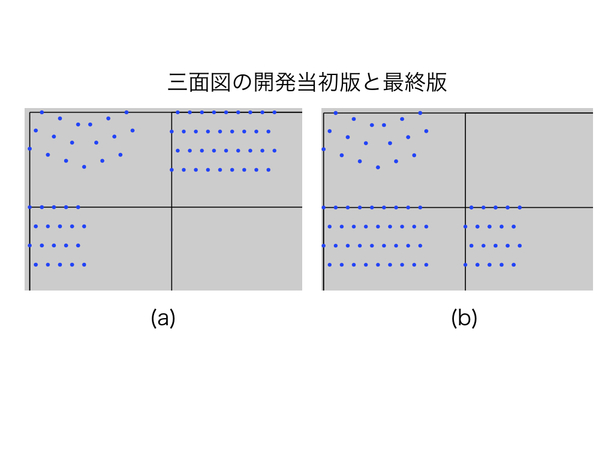
\includegraphics[width=10cm,bb= 0 0 737 553]{../figs/./boundary_narita.014.jpeg}
\caption{POSCAR\_2223を表示した三面図の(a)開発当初版と(b)最終版.}
\label{default}\end{center}\end{figure}
